\begin{myConceptSteps}{To determine if a relation represented as the graph is a function\dots}
    \myStep{inspect the graph}{%
        Look closely at the graph of the relation.
    }
    \myStep{vertical lines}{%
        Are there any vertical lines 
        that {\bfseries\itshape intersect the graph} in more than one place?
    }
    \myStep{Vertical Line Test}{%
        If so, 
        the relation {\bfseries\itshape is not a function}.
        Otherwise, the relation {\bfseries\itshape is a function}.
    }
\end{myConceptSteps}


\begin{myExample}{
    Determine if this relation is a function. Explain your answer.
    \begin{center}
        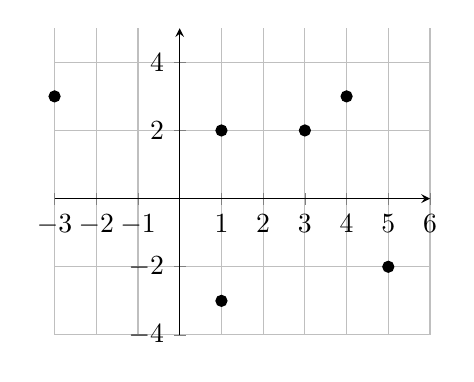
\begin{tikzpicture}
            \begin{axis}[
                width=2.5in,
                grid=both,
                axis x line = middle,axis y line = middle,
                % axis equal image,
                % minor tick num=1,
                xtick distance = 1, ytick distance = 2,
                xmin = -3, xmax=6,
                ymin = -4, ymax=5,
                ]
                \addplot[
                    only marks,
                    mark=*,
                    % mark size = 0.15cm,
                    ] coordinates { (-3,3) (1,2) (3,2) (5,-2) (1,-3) (4,3) };
            \end{axis}
        \end{tikzpicture}
    \end{center}
}
    \vspace{1in}
\end{myExample}

\begin{myExample}{
    Are these functions? Explain why or why not.
    \begin{center}
        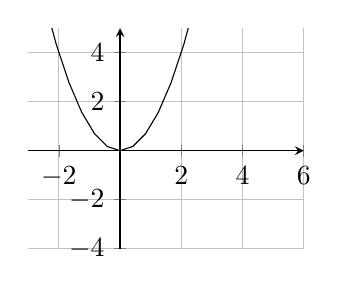
\begin{tikzpicture}
            \begin{axis}[
                width=2in,
                grid=both,
                axis x line = middle,axis y line = middle,
                % axis equal image,
                % minor tick num=1,
                % xtick distance = 1, ytick distance = 2,
                xmin = -3, xmax=6,
                ymin = -4, ymax=5,
                ]
                \addplot[no marks] expression { x^2 };
            \end{axis}
        \end{tikzpicture}
        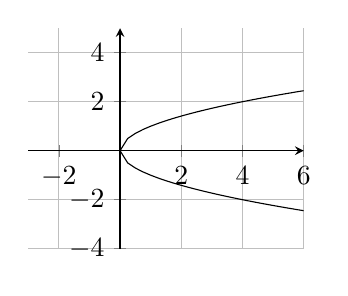
\begin{tikzpicture}
            \begin{axis}[
                width=2in,
                grid=both,
                axis x line = middle,axis y line = middle,
                % axis equal image,
                % minor tick num=1,
                % xtick distance = 1, ytick distance = 2,
                xmin = -3, xmax=6,
                ymin = -4, ymax=5,
                ]
                \addplot[no marks,domain=0:6] expression { sqrt(x) };
                \addplot[no marks,domain=0:6] expression { -sqrt(x) };
            \end{axis}
        \end{tikzpicture}
        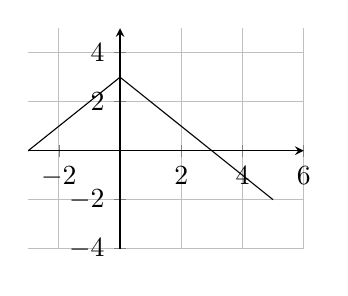
\begin{tikzpicture}
            \begin{axis}[
                width=2in,
                grid=both,
                axis x line = middle,axis y line = middle,
                % axis equal image,
                % minor tick num=1,
                % xtick distance = 1, ytick distance = 2,
                xmin = -3, xmax=6,
                ymin = -4, ymax=5,
                ]
                \addplot[no marks] expression { -abs(x) + 3 };
            \end{axis}
        \end{tikzpicture}
        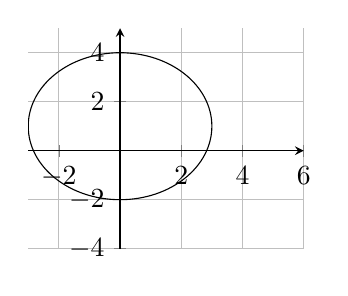
\begin{tikzpicture}
            \begin{axis}[
                width=2in,
                grid=both,
                axis x line = middle,axis y line = middle,
                % axis equal image,
                % minor tick num=1,
                % xtick distance = 1, ytick distance = 2,
                xmin = -3, xmax=6,
                ymin = -4, ymax=5,
                ]
                \draw (axis cs:0,1) circle [radius=3];
            \end{axis}
        \end{tikzpicture}
    \end{center}
}
    \vspace{3in}
\end{myExample}
